% Introduce the chapters contents
%   Previous PyCBC Live Ranking Statistic
%   New Additions
%   PSD Var
%   Template Fits
%   Testing - Injection Tests
%   Sensitivity Increase
%   Investigating decreases in sensitivity
%        Templates with high spin, high mass, false alarms

In this chapter we discuss the improvements made to the PyCBC Live search's ranking statistic which has enabled an increase in the sensitivity of the live search of over 30\%. We will discuss the new additions to the ranking statistic and how these have been adapted for the live search.

\section{\label{live-previous-stat}Previous Ranking Statistic}

As mentioned in~\ref{sec:live-ranking-statistic} PyCBC Live used the same ranking statistic during both the third observing run and the first half of the fourth observing run.

The ranking statistic can be split into two components: a single trigger ranking statistic and a coincident trigger ranking statistic. The single trigger ranking statistic used in PyCBC Live was \verb|newsnr_sgveto|, where \verb|newsnr| refers to the calculation of a new SNR value that has been weighted by the chisq value calculated using the Allen chisq and, \verb|sgveto| is the same re-weighting but for another chisq called the sine-gaussian chisq.

The coincident ranking statistic used was \verb|phasetd| which is the simplest coincident ranking statistic, checking only phase and time consistency of the triggers in separate detectors to ensure they arrived within the physical light travel time and with the same phase state.

\section{\label{live-new-additions}New Additions}

To improve the ranking statistic we have included two new components which are currently used in the PyCBC offline ranking statistic: PSD variation and template fits. These two components have been previously described in sections~\ref{sec:psd-variation}~\&~\ref{sec:template-fitting}.

\subsection{\label{live-psd-var}PSD Variation in Live}

% Section introduction
We have described the theory of PSD variation in section~\ref{sec:psd-variation} and in this section we will describe the implementation of PSD variation in the live search and how this differs from that of the offline search.

% Brief explanation of PSD variation
The PSD measures the power distribution of the data in the frequency domain, when this PSD is inaccurate it can cause inaccurately measured SNR values for a trigger. PSD variation is a measure of the difference between the true PSD of the data and the estimated PSD being used by the search.

% PSD variation in offline
The PyCBC offline search for gravitational waves searches through 512 seconds of data in each chunk. The PSD for this chunk is measured once and used for the whole stretch of time, this can be inaccurate for different points of time in the whole chunk. The offline search therefore measures the PSD variation at each second and when a trigger is found the variation value is found by interpolating between the two nearest seconds.

% Difference between offline and live
The PyCBC live search in contrast maintains a buffer of 256 seconds of data, rolling the newest eight seconds on as the oldest eight second are rolled off. The PSD of this data is measured and the neutron star binary distance is calculated, the PSD is then re-estimated regularly and if the neutron star binary distance of a newly estimated PSD is greater than a 1\% difference to the current PSD then the current PSD is updated to this new PSD. This reduces the effect of a poorly estimated PSD but there is still some potential for non-stationary data to effect the search. 

% How we calculate the PSD var in live?
The offline search computes the PSD variation values for the whole chunk in one go. If the live search were to do the same it would have to compute the PSD variation values every eight seconds for the whole 256 second chunk of data. This would mean that each second would be calculated 32 times as it makes its way through the buffer, wasted computing resources and introducing lag to the search. Instead, the live search only calculates the PSD variation for the latest eight seconds of data, as this is the same time when there will any new triggers for the PSD variation to get assigned to. These PSD variation values are then saved with the triggers and the memory is re-allocated for the next set epoch of the search.

\subsection{\label{live-template-fits}Template Fits}

The offline search takes the previous week (CHECK) of triggers and create the statistic files required for the template fits. This process is identical in the live search's implementation of the template fits except for the triggers need to be collated from the individual trigger files produced every eight seconds and then they need to be converted to the format required to produce the template fits files.
%
\begin{figure}
  \centering
  \begin{minipage}[t]{1.0\linewidth}
  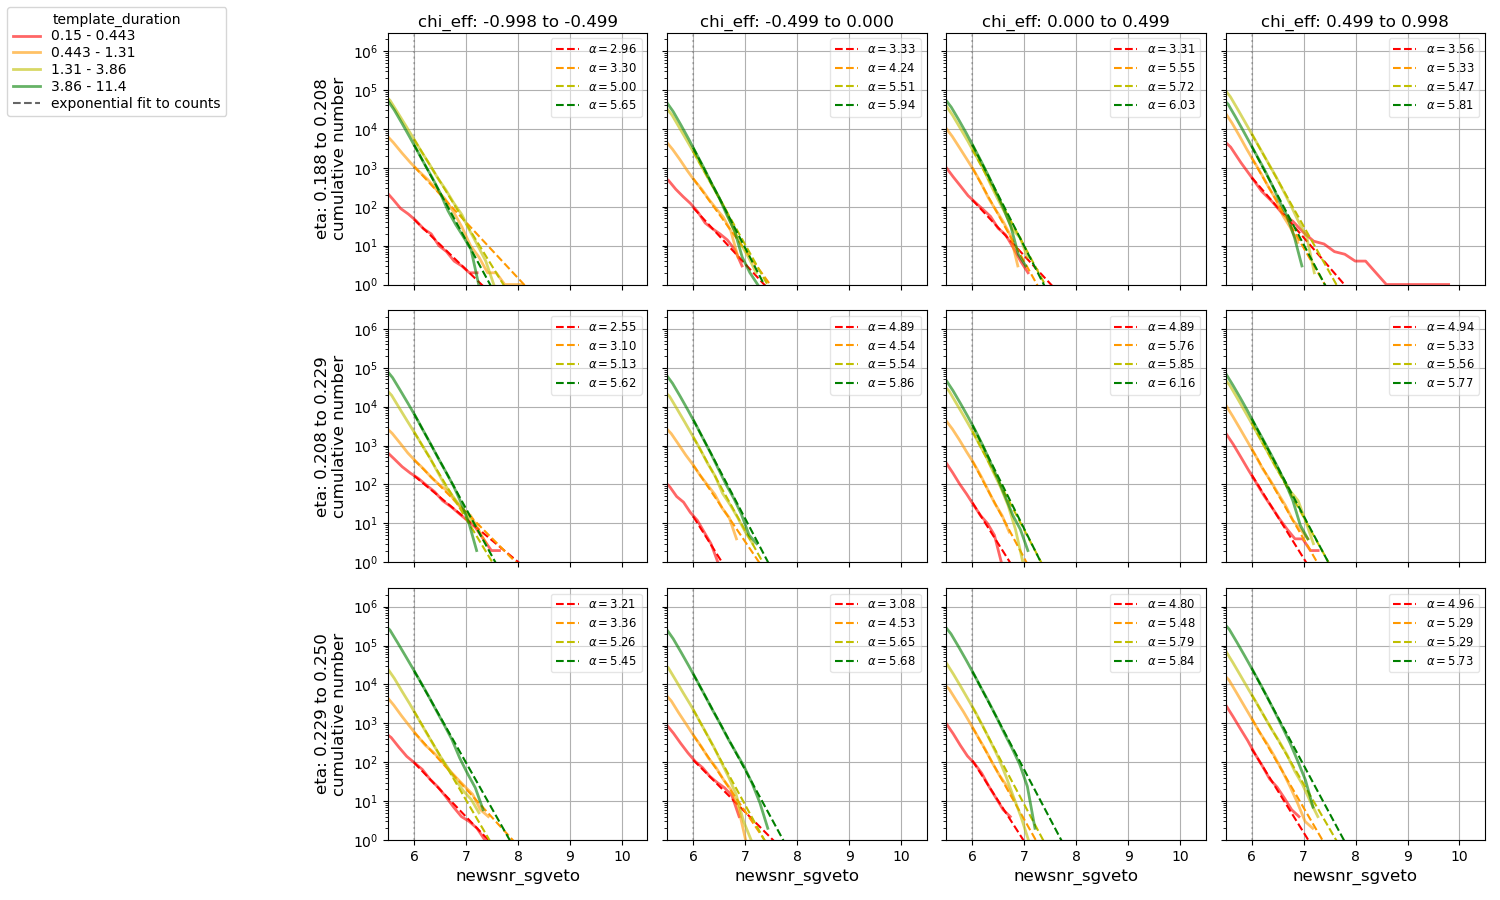
\includegraphics[width=0.49\textwidth]{images/pycbclive/H1-template_fits.png}
  \hspace{0.01\linewidth}
  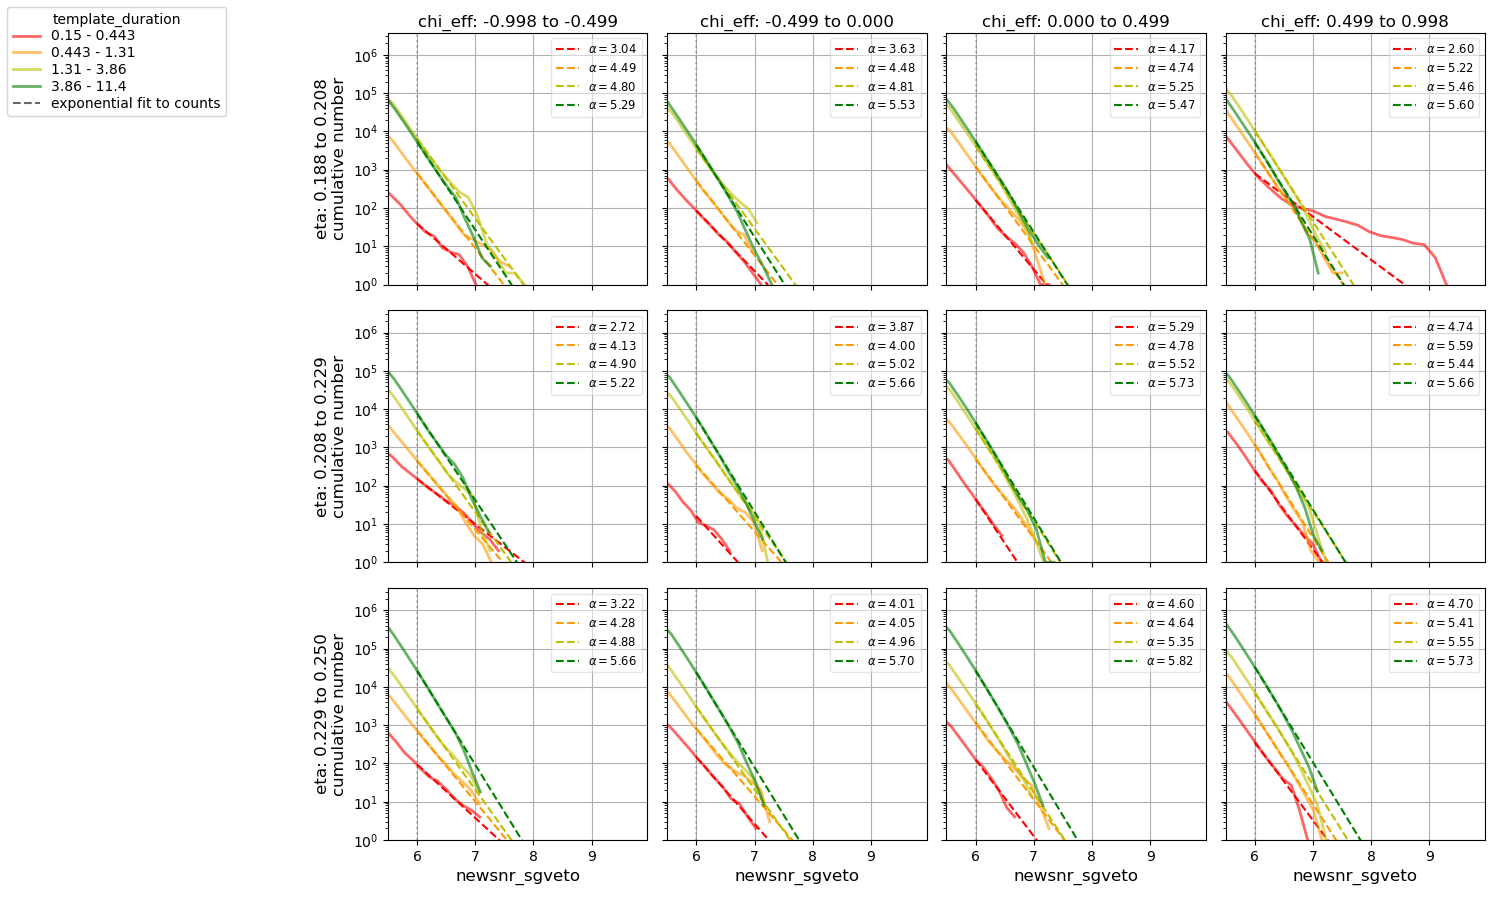
\includegraphics[width=0.49\linewidth]{images/pycbclive/L1-template_fits.png}
  \end{minipage}
  \caption{}
  \label{fig:pycbclive-fits}
\end{figure}
%
Figure~\ref{fig:pycbclive-fits} shows the associated fits made by the injection testing we did to measure the increase in sensitivity. These fits show good agreement to the exponential in the majority of the template bins except for the top-right for both H1 and L1 where there is an excess of high SNR triggers for these high-chieff, low eta and very short duration BBH templates.

\section{\label{sec:pcycblive-sensitivity-improvements}Sensitivity Improvements}

We measure improvement to the live search by performing injection set tests. The injection sets are made up of thousands of gravitational wave signals that are injected at a rate of approximately one every 100 seconds. We run two 'live' searches for gravitational waves, one with the old ranking statistic and one with the new ranking statistic which includes the additions of both PSD variation and template fitting.

The injection set used for this test is made up entirely of BBH signals to reduce the size of the template bank required~(CITE R\&P PAPER FOR O3), there is a limit to the amount of memory a user can request for this pseudo-live search and therefore we couldn't initially test these changes on the full pycbc live template bank. The template bank of 15436 templates covers the BBH signal parameter space and is described in this paper~(CITE O3 BBH PAPER?). 

The gravitational wave data used was a two week period of O3b where the first week was used to generate the template fits and the second week was used to test the fits. The injected gravitational wave data was created before the live searches were run and both searches were run on exactly the same data. While this search is emulating the live search it will very simply wait for new data before it moves forwards by eight seconds, if this data already exists (in the form of pregenerated data) then it will perform the processing as fast as it can. Therefore, a running the live search over a week of data does not take a whole week but it can take as little as 24 hours.

Once both searches have completed we can count the number of injections found by both searches. Theoretically the searches should both observe the exact same number of injections with almost identical triggers due to their nature but, computing isn't always perfect and therefore the searches observed slightly different amounts of time during the second week. This means that a simple count of injections found cannot be done, we need to isolate the injections seen in jointly observed time between the two searches.

This produced a list of injections seen by both searches in which we can directly compare the false alarm rate (or inverse false alarm rate, IFAR) of each injection to see if there has been an improvement. Each of these events is a real gravitational wave signal so we hope to see every single injection with a large IFAR value to indicate that the changes to the ranking statistic has improved the sensitivity of the search. Figure~\ref{fig:pycbclive-ifar-vs-ifar} displays the change in IFAR for each injection with the new statistic (colloquially referred to as 'fits') on the y-axis and the x-axis the old statistic IFAR values.
%
\begin{figure}
       \centering
    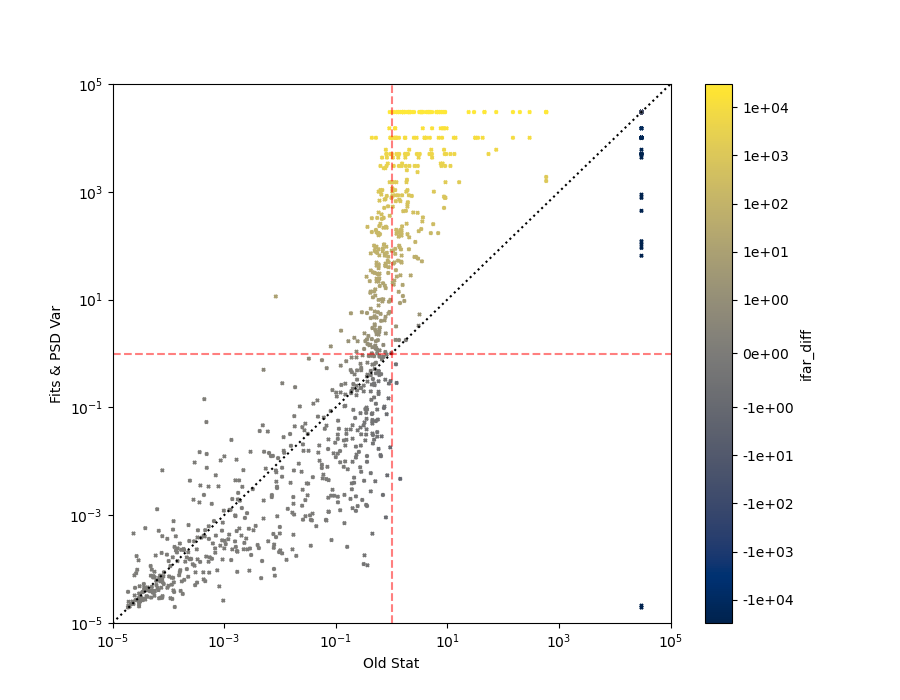
\includegraphics[width=1.2\textwidth]{images/pycbclive/fits_vs_old_colour.png}
    \caption{}
    \label{fig:pycbclive-ifar-vs-ifar}
\end{figure}
%
Within figure~\ref{fig:pycbclive-ifar-vs-ifar} we have plotted a vertical and horizontal dotted line at an IFAR of 1 year to indicate a commonly chosen IFAR limit of where an event would be considered 'real'. Therefore this figure can be split into four quadrants: top-left, injections originally missed below the IFAR threshold and now found above it; top-right, injections found in both searches; bottom-left, injections below the threshold by both searches; bottom-right, injections originally found above the IFAR threshold but missed with the new statistic. Another line has been plotted at y=x, injections above this line (in the top-left) have been found with a larger IFAR with the new statistics and injections below (in the bottom-right) have been found with a lower IFAR with the new statistic.

We have investigated all injections in the bottom-right quadrant and have found discrepancies in why these have been down-ranked which needs further investigation.

To measure the sensitivity improvements of the new statistic we count the number of injections found with IFAR over a certain number for both searches. If we do this for a range of IFAR values then we can build up an image of the sensitivity increase when using the new statistic. Figure~\ref{fig:pycbclive-sensitivity} shows this ratio of new statistic over old statistic.
%
\begin{figure}
       \centering
    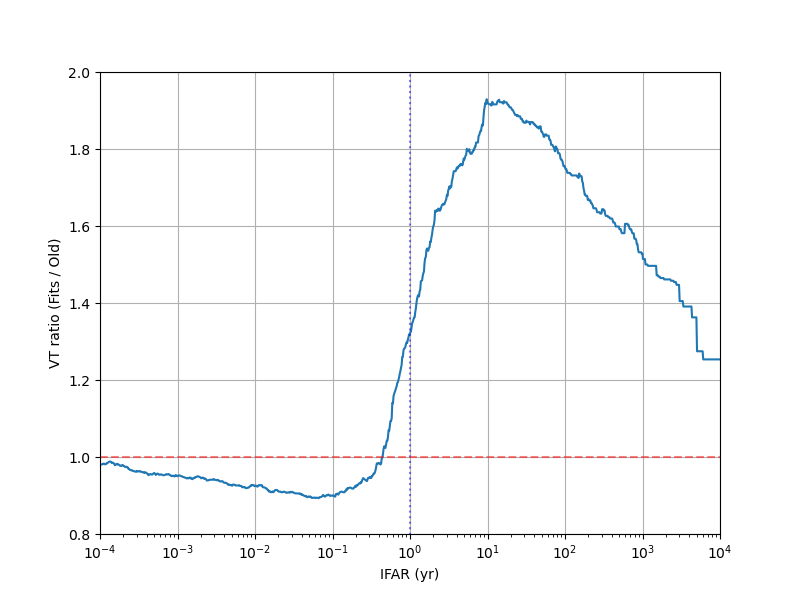
\includegraphics[width=1.0\textwidth]{images/pycbclive/ratio.png}
    \caption{}
    \label{fig:pycbclive-sensitivity}
\end{figure}
%
The new statistic at an IFAR of 1 year can be seen to have found approximately 35\% more gravitational wave signals with an IFAR greater than 1 year. This is a large increase and demonstrates the benefit of adding the PSD variation and templates fits to the live search.

\section{\label{pycbclive-ignoring-psdvar}Ignoring PSD Variation}

Figure~\ref{fig:pycbclive-ifar-vs-ifar} shows a number of outlier injections which have been found with a much lower IFAR in the search with the new statistic when compared to the old statistic IFAR. This is not desirable, especially when concerning the regions toward the right hand side of the figure where we initially observed the injection with a very high significance and do not want to miss this with the new statistic.

The first avenue of exploration is with the new additions made with the new statistic. These were split into the inclusion of PSD variation and template fitting. We already had reservations using the PSD variation in live due to the nature of the live search and its ever adjusting PSD so we can remove the PSD variation contribution to the ranking statistic and check the IFARs of the injections with template fitting only. The IFAR vs IFAR figure for fitting only and the old statistic can be seen in figure~\ref{fig:pycbclive-fits-only-ifar-vs-ifar}.
%
\begin{figure}
       \centering
    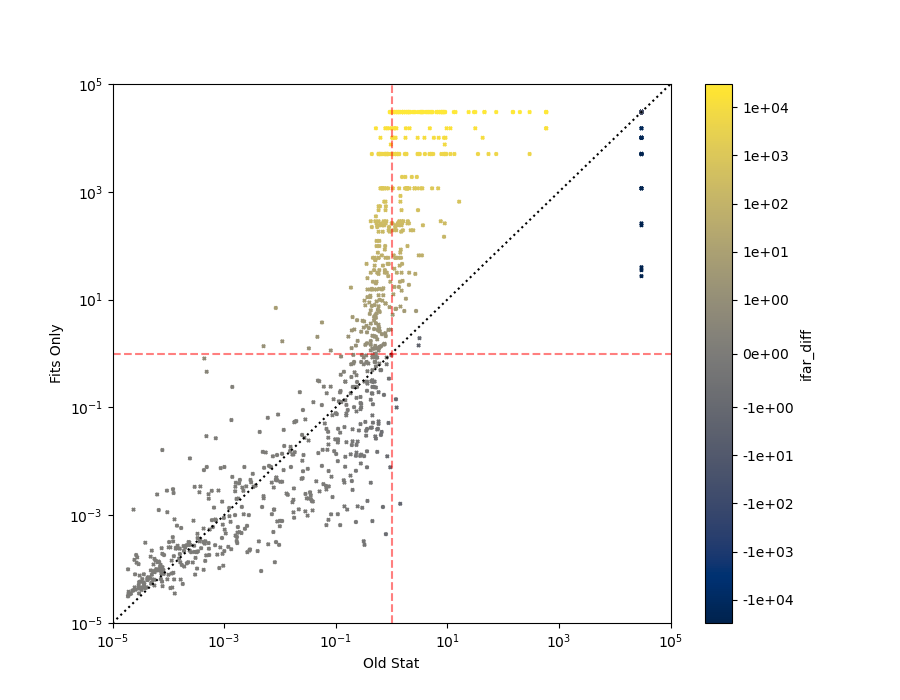
\includegraphics[width=1.2\textwidth]{images/pycbclive/ifar_vs_ifar_fits_only_old.png}
    \caption{}
    \label{fig:pycbclive-fits-only-ifar-vs-ifar}
\end{figure}
%
When compared to figure~\ref{fig:pycbclive-ifar-vs-ifar} we can see the problematic injections in the bottom right corner of the figure have been removed. We can produce the sensitivity plots for both a comparison between the template fitting only statistic vs old statistic and the template fitting \& PSD variation vs template fitting only searches.
%
\begin{figure}
  \centering
  \begin{minipage}[t]{1.0\linewidth}
  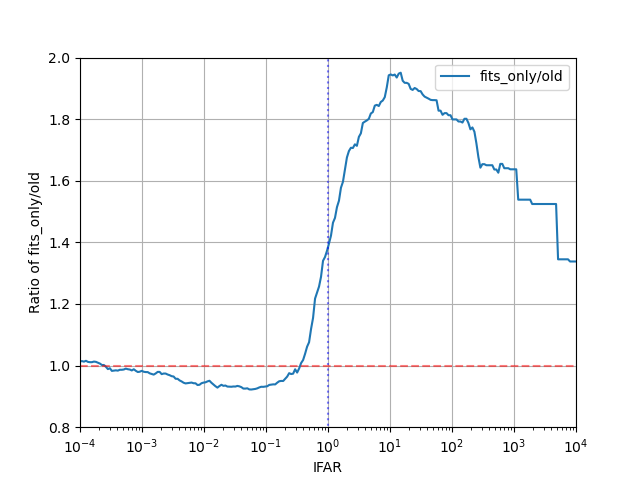
\includegraphics[width=0.49\textwidth]{images/pycbclive/fo_vs_o.png}
  \hspace{0.01\linewidth}
  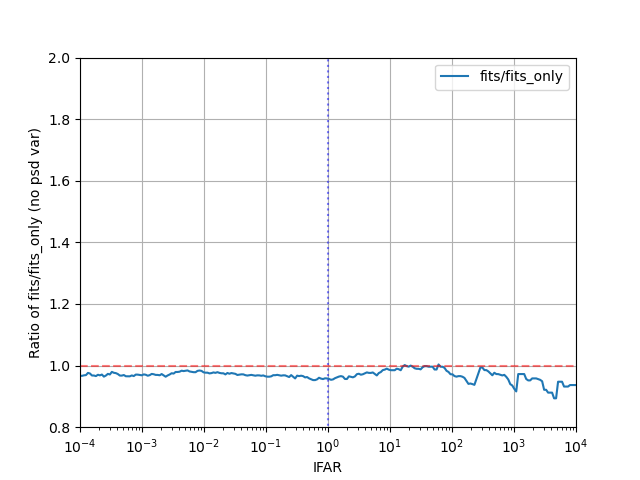
\includegraphics[width=0.49\linewidth]{images/pycbclive/f_vs_fo.png}
  \end{minipage}
  \caption{}
  \label{fig:pycbclive-sensitivity-comparisons}
\end{figure}
%
Figure~\ref{fig:pycbclive-sensitivity-comparisons} (left) shows a marginal increase in sensitivity at the lower IFARs when ignoring PSD variation and (right) shows a clear decrease in sensitivity when including the PSD variation in the new statistic search. Therefore we made the choice to not use PSD variation in the PyCBC Live statistic going forward.

\section{\label{pycbclive-false-alarms}Investigating Downranked Regions}

While we have a sensitivity increase (shown by figure~\ref{fig:pycbclive-sensitivity-comparisons}) the IFAR vs IFAR plot in figure~\ref{fig:pycbclive-fits-only-ifar-vs-ifar} shows there are three group of injections that we need to investigate and understand before we can claim this new statistic is ready to be used in the PyCBC Live search. These three regions are highlighted in figure~\ref{fig:pycbclive-region-highlight}.
%
\begin{figure}
       \centering
    \includegraphics[width=1.2\textwidth]{images/pycbclive/ifar_vs_ifar_regions.png}
    \caption{}
    \label{fig:pycbclive-region-highlight}
\end{figure}
%
The first region to investigate is in the top-right corner of the figure~\ref{fig:pycbclive-region-highlight}. These are injections that were found with the maximum significance by the old statistic but they have been downranked by the inclusion of template fitting in the ranking statistic. While they have been downranked, they are still all found with a high significance and there is no chance they will be missed. This region contains X injections and the primary cause of the downranked significance is due to Y.

The next region is the injections which have been found by the old statistic with an IFAR greater than 1 year but missed by the search which includes template fitting. These are found in the bottom-right grid in figure~\ref{fig:pycbclive-region-highlight}. This region contains X injections and upon investigation we can see that the cuase of this downranking is Y.

The final region we are investigating is those injections which were marginally missed in when using the old statistic, between an IFAR of 0.1 and 1 years, and then were further downranked by including template fitting in the statistic. This is an important region because these are the signals which are close to the IFAR threshold and we want to recover these with an improved statistic. Upon investigating these X (number of) injections we can see that the reason they are downranked is due to Y (most are found with the same template but the template is high mass/high spin/ not well fit).